\documentclass[11pt,a4paper,openany]{book}
\usepackage[margin=24mm]{geometry}
\usepackage{fontspec}
\IfFontExistsTF{Noto Serif}{\setmainfont{Noto Serif}}{\setmainfont{DejaVu Serif}}
\usepackage{amsmath,amssymb,tikz,enumitem,microtype}
\usepackage[hidelinks]{hyperref}
\setlength{\parindent}{0pt}
\setlength{\parskip}{6pt}
\setlist[enumerate]{leftmargin=*,itemsep=8pt}
\setlength{\emergencystretch}{2em}

\renewcommand{\contentsname}{Contents}
\begin{document}
\title{V-TALENT 2045\\ PHY201-B --- Differential equations and complex numbers\\\large Level 2 \textbar{} Mathematics for Physics}
\author{Dr. Dang Minh Tuan -- TS. Đặng Minh Tuấn}
\date{2026 \textbar{} Draft v1.0}
\maketitle
\tableofcontents
\chapter*{How to study}
Grades 10–12 / Olympiad bridge. Prerequisites: PHY201-A, algebra and trigonometry. Develop ODEs from conservation laws and validate the model before solving.

Predict first; draw a model; reproduce worked examples without looking; solve independently and check the solutions at the back. Original teaching content; source links are further reading, not copied text. Draft pending independent review.
\chapter{First-order ODEs and relaxation}
\section{Learning objectives}
Derive separable and linear first-order models; enforce initial conditions and identify time constants.
\section{Theory and derivations}
An ordinary differential equation constrains an unknown function and its derivatives. For $\dot y=-ky$, $k>0$, the nonzero solutions follow from $dy/y=-k\,dt$: $\ln|y|=-kt+C$, thus $y=y_0e^{-kt}$. The zero solution must also be retained. A time constant $\tau=1/k$ has time units, and after one $\tau$ the deviation falls to $1/e$ of its initial value. For $\dot y=-k(y-y_\infty)$ apply the same method to $z=y-y_\infty$.

For $y'+p(t)y=q(t)$ the integrating factor $\mu(t)=e^{\int_{t_0}^{t}p(s)\,ds}$ yields $(\mu y)'=\mu q$. Hence $y(t)=\mu^{-1}(t)[y_0+\int_{t_0}^t\mu(s)q(s)\,ds]$. The equation is linear in y and y', even when the coefficients vary in time. This is not a universal method for nonlinear ODEs. A solution is verified by substitution and its initial condition, not by its appearance.

For an ideal series RC circuit with a constant source V, Kirchhoff's law gives $R\dot q+q/C=V$. Thus $q(t)=CV+(q_0-CV)e^{-t/(RC)}$, and $I=\dot q$. The time constant RC has seconds as units. For $q_0=0$, capacitor voltage rises toward V and current decays from V/R. During discharge set source V=0. Capacitor voltage is continuous for finite current.

Linear drag during vertical fall (downward positive) yields $m\dot v=mg-bv$, so $v=v_T+(v_0-v_T)e^{-bt/m}$ with $v_T=mg/b$. This is an ideal linear-resistance regime. For quadratic drag $m\dot v=mg-cv|v|$ the relaxation is not generally a single exponential. A terminal speed balances forces, not a cessation of motion.
\begin{center}
\begin{tikzpicture}[x=.85cm,y=3cm]\draw[->](0,0)--(5.5,0)node[right]{$t/\tau$};\draw[->](0,0)--(0,1.2)node[above]{$U_C/V$};\draw[dashed](0,1)--(5,1);\draw[blue,thick,domain=0:5,samples=60]plot(\x,{1-exp(-\x)});\draw[dashed](1,0)--(1,.632)--(0,.632);\node[left]at(0,.632){$.632$};\end{tikzpicture}
\end{center}
\section{Worked examples}
\subsection*{Example 1.1}
An initially uncharged 1000 microfarad capacitor charges through 2 kilohms from 6 V. Find time constant, voltage and current at 2 s.

\textbf{Solution.} $\tau=2000(0.001)=2$ s. $U_C=6(1-e^{-1})=3.793$ V. $I=(6/2000)e^{-1}=1.104$ mA.
\subsection*{Example 1.2}
Solve y'+2y=4t, y(0)=1.

\textbf{Solution.} A particular solution $2t-1$ satisfies the equation; homogeneous $Ce^{-2t}$. Initial value gives C=2, hence $y=2t-1+2e^{-2t}$. Substitute: $y'+2y=4t$.
\section{Investigation}
Use SIM-D01 to vary R and C, measure the time to 63.2 percent of a voltage step, and plot normalized voltage against t/(RC). Compare curves. Use simulation only or a supervised low-voltage circuit.
\section{Modern application and transfer}
A first-order temperature model for a chip is Cth dT/dt=P-(T-Ta)/Rth, giving thermal time constant Rth Cth. A power step changes equilibrium by PRth. This lumped model is useful when internal temperature gradients are small; multiple thermal nodes may be necessary otherwise.
\section{Source-guided reading}
SJ §§13.1–13.1.1, pp. 51–52 (ODE and RC); Chasnov, Differential Equations, via Kevin S. Huang (further reading).
\section{Independent practice}
\begin{enumerate}
\item \textbf{PHY201-B-1.1}. Solve dy/dt=-3y, y(0)=8; find half-life.
\item \textbf{PHY201-B-1.2}. A 4 V charged capacitor discharges with RC=0.5 s. Find voltage after 1 s.
\item \textbf{PHY201-B-1.3}. A 0.2 kg body falls from rest with b=0.1 kg/s and g=10 m/s\textsuperscript{2}. Find terminal speed and speed after 2 s.
\item \textbf{PHY201-B-1.4}. Solve y'+y=e^(-t), y(0)=0, and verify.
\end{enumerate}
\chapter{Complex numbers, Euler form and phasors}
\section{Learning objectives}
Convert between rectangular and polar forms; use complex exponentials for sinusoidal signals without confusing real observables with complex representations.
\section{Theory and derivations}
Define $i^2=-1$. For $z=a+ib$, conjugate $z^*=a-ib$ and magnitude $|z|=\sqrt{a^2+b^2}$. Since $zz^*=|z|^2$, division by a nonzero complex number uses its conjugate. In polar form $z=re^{i\phi}$ with $r\ge0$; arguments are defined modulo $2\pi$ and undefined at zero. Euler's relation $e^{i\phi}=\cos\phi+i\sin\phi$ follows from the power series for exponential, sine and cosine. Multiplication adds arguments and multiplies magnitudes.

A real harmonic signal can be represented as $x(t)=\operatorname{Re}(Xe^{i\omega t})$ with phasor $X=Ae^{i\phi}$. Differentiation corresponds to multiplication by $i\omega$ and integration of a nonzero-frequency sinusoidal component to division by $i\omega$. The complex notation is a calculation device: physical displacement or voltage is the real part. The method applies directly to linear time-invariant systems in sinusoidal steady state; initial transients require separate solutions.

For two sinusoids with the same angular frequency, add phasors: $x_1+x_2=\operatorname{Re}[(X_1+X_2)e^{i\omega t}]$. Different frequencies cannot in general be replaced by a single constant phasor. For $X_1=A$ and $X_2=Ae^{i\delta}$, the resulting amplitude is $2A|\cos(\delta/2)|$. This phase dependence underlies interference and signal cancellation.
\begin{center}
\begin{tikzpicture}[scale=.9]\draw[->](-.5,0)--(4,0)node[right]{Re};\draw[->](0,-.5)--(0,3.5)node[above]{Im};\draw[->,very thick,blue](0,0)--(3,2)node[above]{$z$};\draw[dashed](3,2)--(3,0)(3,2)--(0,2);\node[below]at(3,0){$a$};\node[left]at(0,2){$b$};\draw(1,0)arc(0:33.69:1);\end{tikzpicture}
\end{center}
\section{Worked examples}
\subsection*{Example 2.1}
Compute (3+4i)/(1-2i), magnitude and argument quadrant.

\textbf{Solution.} Multiply by $1+2i$: numerator $-5+10i$, denominator 5. Result $-1+2i$, magnitude $\sqrt5$, quadrant II, argument $\pi-\arctan2$.
\subsection*{Example 2.2}
Add x1=3cos(\ensuremath{\omega}t), x2=4cos(\ensuremath{\omega}t+\ensuremath{\pi}/2). Find resultant amplitude and phase.

\textbf{Solution.} $X=3+4i=5e^{i\phi}$, $\phi=\arctan(4/3)$. Thus $x=5\cos(\omega t+\phi)$.
\section{Investigation}
Generate two same-frequency sine curves in a spreadsheet and vary phase difference from 0 to \ensuremath{\pi}. Compare measured maximum amplitude with the phasor prediction.
\section{Modern application and transfer}
Two coherent vibration sources of equal amplitude can partly cancel if controlled with opposite phase. Active vibration and noise control require phase and amplitude estimates at a particular sensor; cancellation at one location does not imply cancellation everywhere.
\section{Source-guided reading}
SJ §13.2.2, p. 52 (complex exponential); SW §1.4 catalogue locator; latter not reopened successfully.
\section{Independent practice}
\begin{enumerate}
\item \textbf{PHY201-B-2.1}. Find (2+i)(1-3i).
\item \textbf{PHY201-B-2.2}. Express z=-1-i in polar form with argument in (-\ensuremath{\pi},\ensuremath{\pi}].
\item \textbf{PHY201-B-2.3}. For x=0.1cos(20t+0.3), obtain the velocity phasor and real velocity.
\item \textbf{PHY201-B-2.4}. Two coherent signals each have amplitude 2 and phase difference 120 degrees. Find combined amplitude.
\end{enumerate}
\chapter{Second-order ODEs: free and damped oscillations}
\section{Learning objectives}
Derive the characteristic equation, distinguish three damping regimes and satisfy two initial conditions.
\section{Theory and derivations}
For mass m attached to an ideal spring k with displacement x from equilibrium and viscous damping b, Newton's law is $m\ddot x+b\dot x+kx=0$. Define $\omega_0=\sqrt{k/m}$ and $\gamma=b/(2m)$; then $\ddot x+2\gamma\dot x+\omega_0^2x=0$. For $b=0$, $x=A\cos\omega_0t+B\sin\omega_0t$; initial displacement and velocity give $A=x_0$, $B=v_0/\omega_0$. Mechanical energy is constant only in the undamped ideal case; with b positive, $\dot E=-b\dot x^2$.

Try $x=e^{rt}$ to obtain $r^2+2\gamma r+\omega_0^2=0$, with roots $-\gamma\pm\sqrt{\gamma^2-\omega_0^2}$. For $\gamma<\omega_0$, define $\omega_d=\sqrt{\omega_0^2-\gamma^2}$, giving $x=e^{-\gamma t}(A\cos\omega_dt+B\sin\omega_dt)$; $A=x_0$, $B=(v_0+\gamma x_0)/\omega_d$. At critical damping $\gamma=\omega_0$, repeated root requires $x=(A+Bt)e^{-\gamma t}$, with $B=v_0+\gamma x_0$. For overdamping two distinct real roots produce $x=Ae^{r_1t}+Be^{r_2t}$. Solve $A+B=x_0$, $r_1A+r_2B=v_0$.

For underdamping, successive same-sign peak magnitudes decrease by $e^{-\gamma T_d}$ with $T_d=2\pi/\omega_d$. The logarithmic decrement $\ln(|x_n|/|x_{n+1}|)=\gamma T_d$ estimates damping. Peaks must be separated by one full period, not half a period. Real friction can be Coulomb-like or nonlinear; an exponential envelope is a prediction of viscous damping, not a universal fact.
\begin{center}
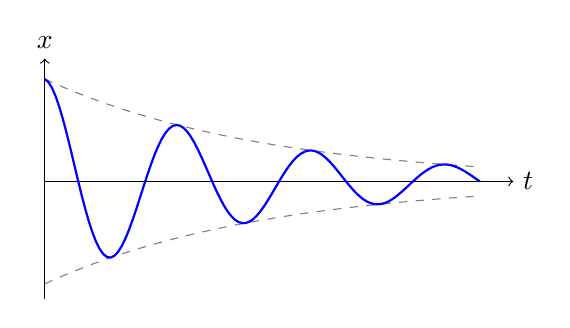
\begin{tikzpicture}[x=.85cm,y=1.3cm]\draw[->](0,0)--(7,0)node[right]{$t$};\draw[->](0,-1.15)--(0,1.2)node[above]{$x$};\draw[dashed,gray,domain=0:6.5,samples=60]plot(\x,{exp(-.3*\x)});\draw[dashed,gray,domain=0:6.5,samples=60]plot(\x,{-exp(-.3*\x)});\draw[blue,thick,domain=0:6.5,samples=120]plot(\x,{exp(-.3*\x)*cos(180*\x)});\end{tikzpicture}
\end{center}
\section{Worked examples}
\subsection*{Example 3.1}
For m=0.5 kg, k=8 N/m, x0=0.1 m, v0=-0.2 m/s and no damping, find x(t) and amplitude.

\textbf{Solution.} $\omega_0=4$ rad/s. $x=0.1\cos4t-0.05\sin4t$ m; amplitude $\sqrt{0.01+0.0025}=0.1118$ m.
\subsection*{Example 3.2}
Solve x''+4x'+4x=0 with x(0)=1 and x'(0)=0.

\textbf{Solution.} Repeated root -2. $x=(A+Bt)e^{-2t}$. A=1; $x'(0)=B-2A=0$ gives B=2. Thus $x=(1+2t)e^{-2t}$.
\section{Investigation}
Use SIM-D02 to compare damping ratios 0, 0.3, 1 and 1.5 for equal initial displacement and zero velocity. Identify oscillations, overshoot and settling; do not equate zero crossing with settling.
\section{Modern application and transfer}
A micro-mechanical accelerometer can be modeled as a proof mass on a spring with damping, driven by inertial force. Damping trades oscillatory ringing against response speed. The best damping depends on the required bandwidth, noise and transient tolerance, not a universal optimal number.
\section{Source-guided reading}
SJ §13.2, pp. 52–54; SJ ch. 14; SW ch. 5 catalogue locator.
\section{Independent practice}
\begin{enumerate}
\item \textbf{PHY201-B-3.1}. Find critical b for m=2 kg, k=18 N/m.
\item \textbf{PHY201-B-3.2}. Solve x''+2x'+5x=0, x(0)=0, x'(0)=4.
\item \textbf{PHY201-B-3.3}. Solve x''+5x'+6x=0, x(0)=1, x'(0)=0.
\item \textbf{PHY201-B-3.4}. Successive positive peaks are 8 cm and 4 cm separated by 2 s. Estimate \ensuremath{\gamma} and explain the model assumption.
\end{enumerate}
\chapter{Forced response, resonance and AC circuits}
\section{Learning objectives}
Derive steady-state amplitude and phase; distinguish displacement resonance from current resonance; use impedance and check assumptions.
\section{Theory and derivations}
For $m\ddot x+b\dot x+kx=F_0\cos\omega t$, take $x_{\rm ss}=\operatorname{Re}(Xe^{i\omega t})$. Substitution yields $(k-m\omega^2+ib\omega)X=F_0$, so amplitude $|X|=F_0/\sqrt{(k-m\omega^2)^2+b^2\omega^2}$ and lag $\delta=\arg(k-m\omega^2+ib\omega)$ in $[0,\pi]$ for positive damping and frequency. The general solution also contains the homogeneous transient; only for positive damping does that transient decay.

Minimize the squared denominator by differentiating in $\omega$: derivative $2\omega[2m(m\omega^2-k)+b^2]$. A nonzero displacement peak exists if $b^2<2mk$ and lies at $\omega_r=\sqrt{\omega_0^2-2\gamma^2}$. Otherwise the maximum over nonnegative frequencies occurs at zero. At exactly $\omega_0$ with b positive, displacement lags force by $\pi/2$. For zero damping and exact resonance the bounded steady-state formula fails; a particular solution grows proportional to time.

Using the $e^{i\omega t}$ convention, resistor impedance $Z_R=R$, inductor $Z_L=i\omega L$, capacitor $Z_C=1/(i\omega C)=-i/(\omega C)$. For series RLC, $Z=R+i(\omega L-1/(\omega C))$ and current phasor $I=V/Z$. With fixed source amplitude and R>0, current amplitude is maximal at $\omega_0=1/\sqrt{LC}$ where reactances cancel. This differs from mechanical displacement resonance because current corresponds to a derivative of charge. For peak amplitudes, average power $P=V_0I_0\cos\phi/2=I_0^2R/2$; for RMS amplitudes no factor 1/2 appears.

An RC low-pass filter uses output across C, with transfer function $H=1/(1+i\omega RC)$. Its magnitude is $1/\sqrt{1+(\omega RC)^2}$, phase $-\arctan(\omega RC)$, and cutoff angular frequency $1/(RC)$ at magnitude $1/\sqrt2$. The transfer function assumes an ideal voltage source and negligible loading. This is a bridge from first-order dynamics to signal processing.
\begin{center}
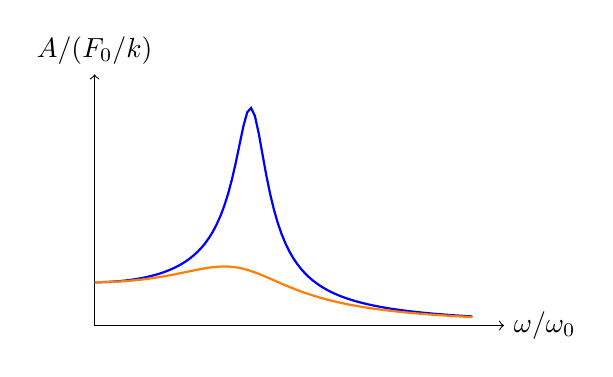
\begin{tikzpicture}[x=2cm,y=.55cm]\draw[->](0,0)--(2.6,0)node[right]{$\omega/\omega_0$};\draw[->](0,0)--(0,5.8)node[above]{$A/(F_0/k)$};\draw[blue,thick,domain=0:2.4,samples=100]plot(\x,{1/sqrt((1-\x*\x)^2+(.2*\x)^2)});\draw[orange,thick,domain=0:2.4,samples=100]plot(\x,{1/sqrt((1-\x*\x)^2+(.8*\x)^2)});\end{tikzpicture}
\end{center}
\section{Worked examples}
\subsection*{Example 4.1}
For m=1 kg, k=100 N/m, b=4 kg/s, F0=2 N, find displacement amplitude and phase lag at \ensuremath{\omega}=10 rad/s; find resonance frequency.

\textbf{Solution.} At 10 rad/s, real denominator zero, imaginary 40: $A=2/40=0.05$ m; lag $\pi/2$. $\gamma=2$, $\omega_r=\sqrt{100-8}=\sqrt{92}\approx9.592$ rad/s.
\subsection*{Example 4.2}
Series RLC has R=10 ohms, L=0.1 H, C=100 microfarads and peak source 5 V. Find resonant frequency and average power there.

\textbf{Solution.} $\omega_0=1/\sqrt{0.1(10^{-4})}=316.23$ rad/s, $f=50.33$ Hz. $I_0=5/10=0.5$ A; $P=I_0^2R/2=1.25$ W.
\section{Investigation}
Use SIM-D03 to sweep normalized frequency at several damping ratios. Find the peak, compare with the predicted shift, and explain why a high peak can be undesirable for structural safety.
\section{Modern application and transfer}
In an ideal RC sensor front end, R=10 kilohms and C=10 nanofarads give RC=0.0001 s and cutoff about 1592 Hz. At 10 kHz the gain is about 0.157. Filtering suppresses high-frequency interference but also attenuates useful fast signals; choose bandwidth based on the measurement goal.
\section{Source-guided reading}
SJ ch. 42, p. 130 (outline only, not full derivation); Swiss ch. 5 and 11 catalogue locators; Chasnov ODE extension.
\section{Independent practice}
\begin{enumerate}
\item \textbf{PHY201-B-4.1}. For \ensuremath{\omega}0=5 rad/s and \ensuremath{\gamma}=1 rad/s, compute displacement resonance frequency.
\item \textbf{PHY201-B-4.2}. For \ensuremath{\omega}0=4 rad/s and \ensuremath{\gamma}=3 rad/s, does a nonzero displacement peak exist?
\item \textbf{PHY201-B-4.3}. At \ensuremath{\omega}=100 rad/s, R=4 ohms, L=0.05 H, C=0.01 F, source peak 10 V. Find impedance, current amplitude and lag.
\item \textbf{PHY201-B-4.4}. An RC low-pass has RC=0.02 s. Find gain and phase at \ensuremath{\omega}=50 rad/s and interpret.
\end{enumerate}
\chapter*{References and simulations}
Tan Chien Hao (2024). \textit{Freshman Physics}.\par
Swiss Physics Olympiad Script, 3rd ed. (2019), catalogue locators pending recheck.\par
\url{https://www.math.ust.hk/~machas/differential-equations.pdf}\par
\url{https://diavn.github.io/truongchuyen/physics-curriculum.html}\par
\url{https://diavn.github.io/truongchuyen/physics-dynamics-lab.html}
\appendix
\chapter{Full solutions}
\section{First-order ODEs and relaxation}
\begin{enumerate}
\item \textbf{PHY201-B-1.1}. $y=8e^{-3t}$; $e^{-3t}=1/2$ gives $t_{1/2}=\ln2/3$.
\item \textbf{PHY201-B-1.2}. $U=4e^{-1/0.5}=4e^{-2}\approx0.541$ V.
\item \textbf{PHY201-B-1.3}. $v_T=mg/b=20$ m/s; $\tau=m/b=2$ s; $v(2)=20(1-e^{-1})=12.64$ m/s.
\item \textbf{PHY201-B-1.4}. Multiply by $e^t$: $(e^ty)'=1$. Integrate: $e^ty=t$, hence $y=te^{-t}$. Derivative $(1-t)e^{-t}$ plus y equals $e^{-t}$.
\end{enumerate}
\section{Complex numbers, Euler form and phasors}
\begin{enumerate}
\item \textbf{PHY201-B-2.1}. $2-6i+i-3i^2=5-5i$.
\item \textbf{PHY201-B-2.2}. $r=\sqrt2$, $\phi=-3\pi/4$, so $z=\sqrt2e^{-3i\pi/4}$.
\item \textbf{PHY201-B-2.3}. $X=0.1e^{0.3i}$; $V=i20X=2e^{i(0.3+\pi/2)}$; $v=-2\sin(20t+0.3)$ m/s.
\item \textbf{PHY201-B-2.4}. $2A|\cos(\delta/2)|=4\cos60^\circ=2$.
\end{enumerate}
\section{Second-order ODEs: free and damped oscillations}
\begin{enumerate}
\item \textbf{PHY201-B-3.1}. $b_c=2\sqrt{mk}=2\sqrt{36}=12$ kg/s.
\item \textbf{PHY201-B-3.2}. Roots $-1\pm2i$. $x=e^{-t}(A\cos2t+B\sin2t)$; A=0, 2B=4, so $x=2e^{-t}\sin2t$.
\item \textbf{PHY201-B-3.3}. Roots -2,-3; $A+B=1$, $-2A-3B=0$, giving A=3,B=-2. $x=3e^{-2t}-2e^{-3t}$.
\item \textbf{PHY201-B-3.4}. $\gamma=\ln(8/4)/2=\ln2/2\approx0.347$ s$^{-1}$. Assumes free linear viscously damped oscillation and same-sign peaks.
\end{enumerate}
\section{Forced response, resonance and AC circuits}
\begin{enumerate}
\item \textbf{PHY201-B-4.1}. $\omega_r=\sqrt{25-2}=\sqrt{23}\approx4.796$ rad/s.
\item \textbf{PHY201-B-4.2}. $\omega_0^2-2\gamma^2=16-18<0$. No; maximum at zero frequency.
\item \textbf{PHY201-B-4.3}. $Z=4+i(5-1)=4+4i$. $|I|=10/(4\sqrt2)=1.768$ A; current lags voltage by $\pi/4$.
\item \textbf{PHY201-B-4.4}. $\omega RC=1$, so gain $1/\sqrt2$, phase $-\pi/4$. This is the cutoff: output peak is 70.7 percent of input peak.
\end{enumerate}
\end{document}
